	
	\subsubsection{Distribuci\'on normal}		
		
		\subsubsection*{Caso 1}
		
		\begin{tabular}{| l | l |}
		\hline
		Parametro & 20 \\
		\hline
		Columna & C2 \\
		\hline
		Valor maximo & 1002 \\
		\hline
		Valor minimo & -671 \\
		\hline
		Distribuci\'on & Normal, Media=200 \\
		\hline
		Selectividad de & Igualdad \\
		\hline
		\end{tabular}
		
		\quad 
		
		\quad 

	\begin{figure}[H]
	  \begin{center}
	    %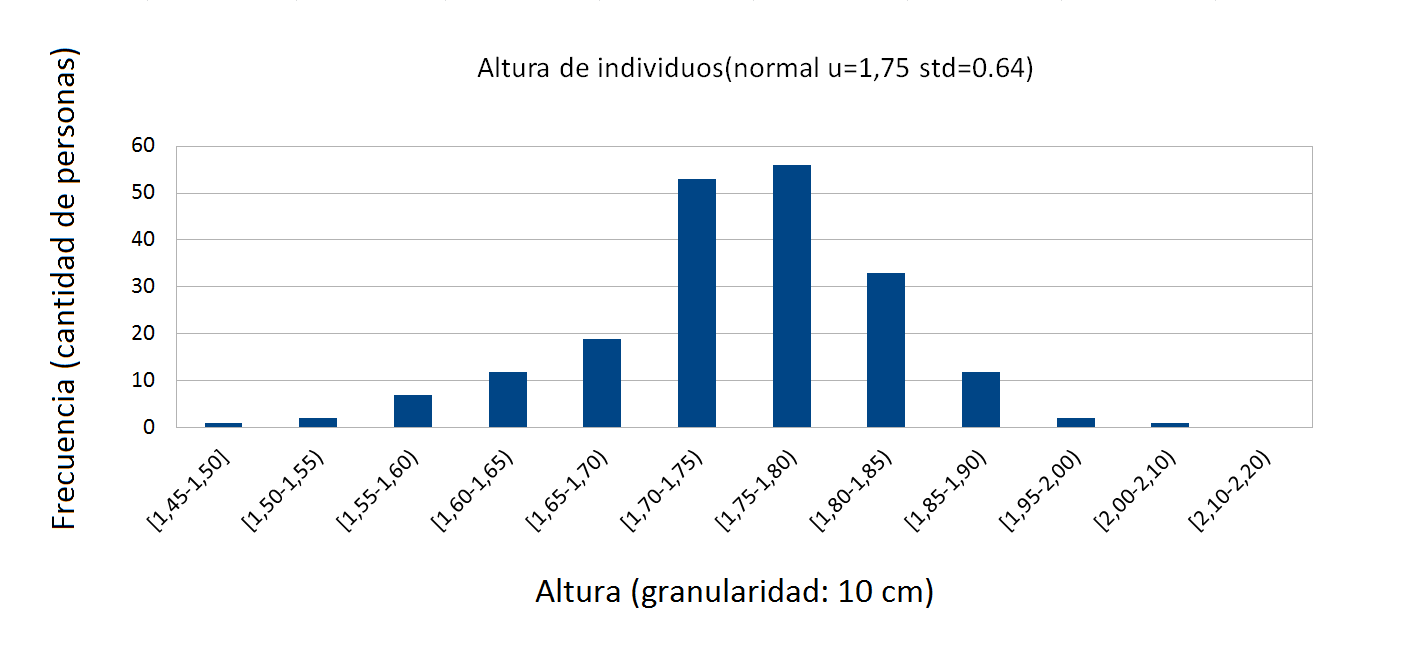
\includegraphics[scale=.41,angle=-90]{imgenes/normal_ejemplo1.png}
	    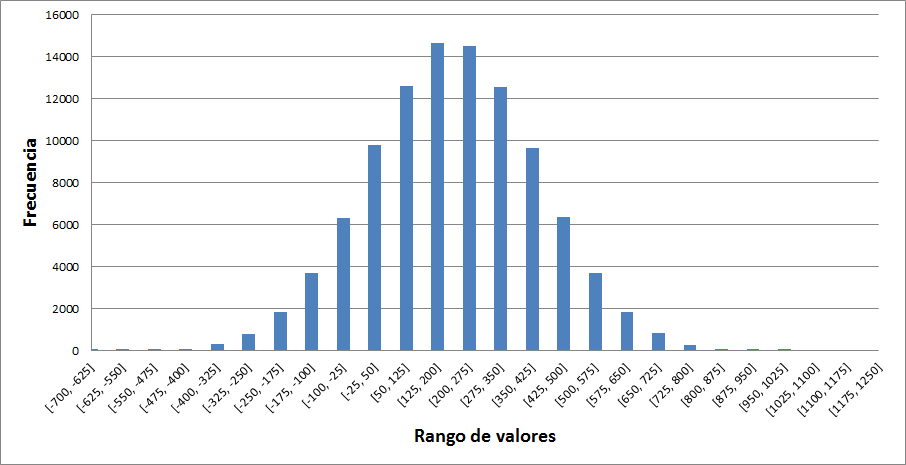
\includegraphics[scale=.60]{imagenes/distro_C2.png}
	    \caption{Gr\'afico de distribuci\'on de la columna C2 del set de datos de la c\'atedra} 
	    \label{fig:(distro_C2}
	  \end{center}
	\end{figure}


	\begin{figure}[H]
	  \begin{center}
	    %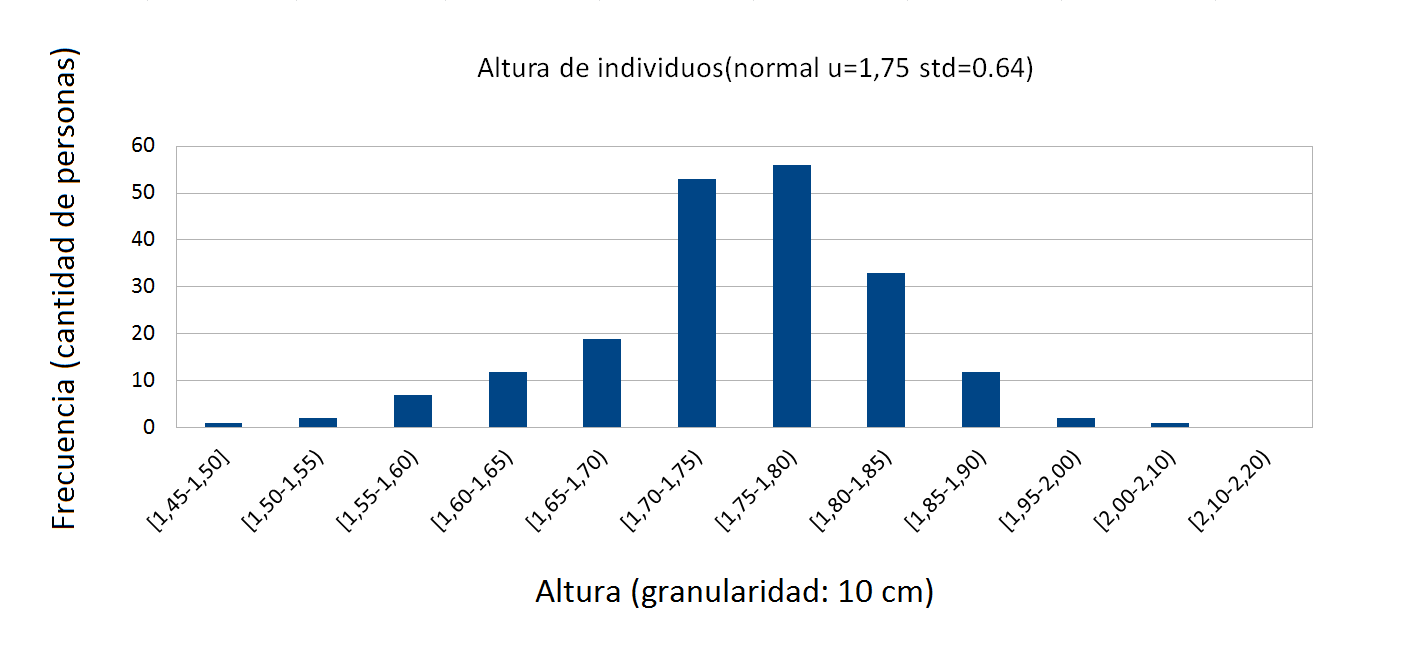
\includegraphics[scale=.41,angle=-90]{imgenes/normal_ejemplo1.png}
	    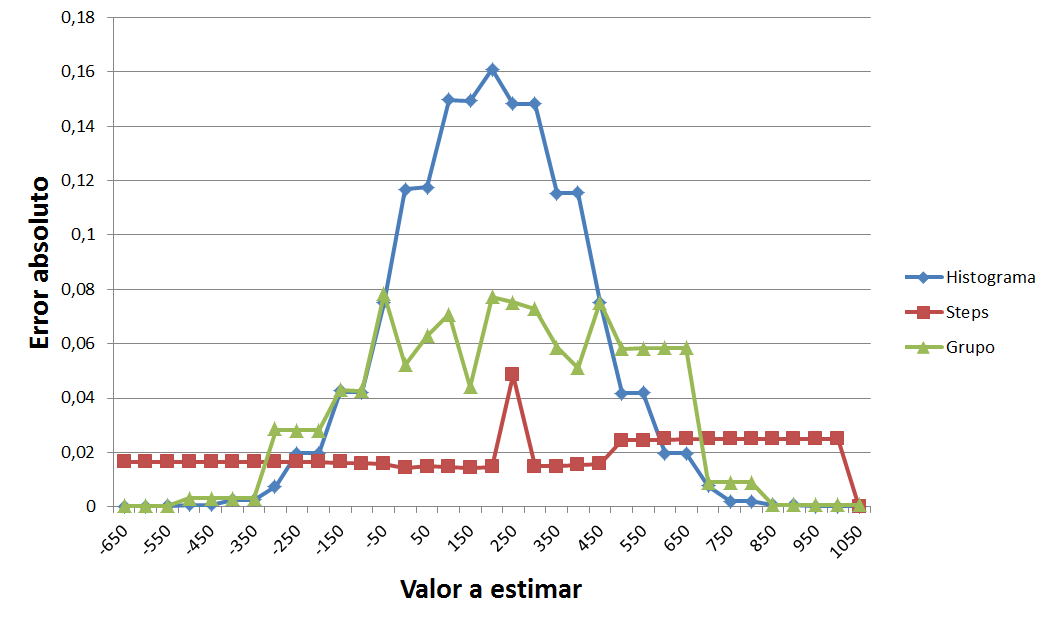
\includegraphics[scale=.55]{imagenes/C2_variando_valor.png}
	    \caption{Errores variando valor a estimar con par\'ametro fijo} 
	    \label{fig:C2_variando_valor}
	  \end{center}
	\end{figure}
		
		En la figura \ref{fig:(distro_C2} se ve la distribucion del set de datos que estamos analizando. Se puede ver como es una distribucion Normal con media 200 y un desv\'io alrededor de 300.
		
		En la gr\'afico de la figura \ref{fig:C2_variando_valor} se ve como, teniendo los par\'ametros de los estimadores fijos, y variando el valor a estimar, el estimador de Distribution Steps obtiene un error constante y bastante chico en todo el rango. Pero el Classic Histogram se comporta mejor en los casos que est\'an por afuera del desv\'io standard de la normal (en este caso, al rededor de 300).
		
		Tambi\'en, se puede ver como el estimador Classic Histogram obtiene errores muy grandes cuando el valor es muy cercano a la media. En la media, se ve como el error llega al m\'aximo.
		
		En cuanto al estimador ideado por el grupo, se ve como al igual que el Histograma Cl\'asico, se obtiene errores muy chicos en valores lejos del desv\'io standard de la normal. A su ves, errores altos en los valores al rededor de la media. Sin embargo, estos errores son inferiores a los obtenidos en el histograma. Esto probablemente se deba a que el estimador del Grupo, es un histograma cl\'asico pero con una re-distribuci\'on en los \textit{bins} con m\'as valores, los cuales en este caso estar\'an cerca de la media.
	
		\subsubsection*{Caso 2}
		
		\begin{tabular}{| l | l |}
		\hline
		Parametro & 20 \\
		\hline
		Columna & C2 \\
		\hline
		Valor maximo & 1002 \\
		\hline
		Valor minimo & -671 \\
		\hline
		Distribuci\'on & Normal, Media=200 \\
		\hline
		Selectividad de & Mayor \\
		\hline
		\end{tabular}

	\quad
	
	\quad 				

	\begin{figure}[H]
	  \begin{center}
	    %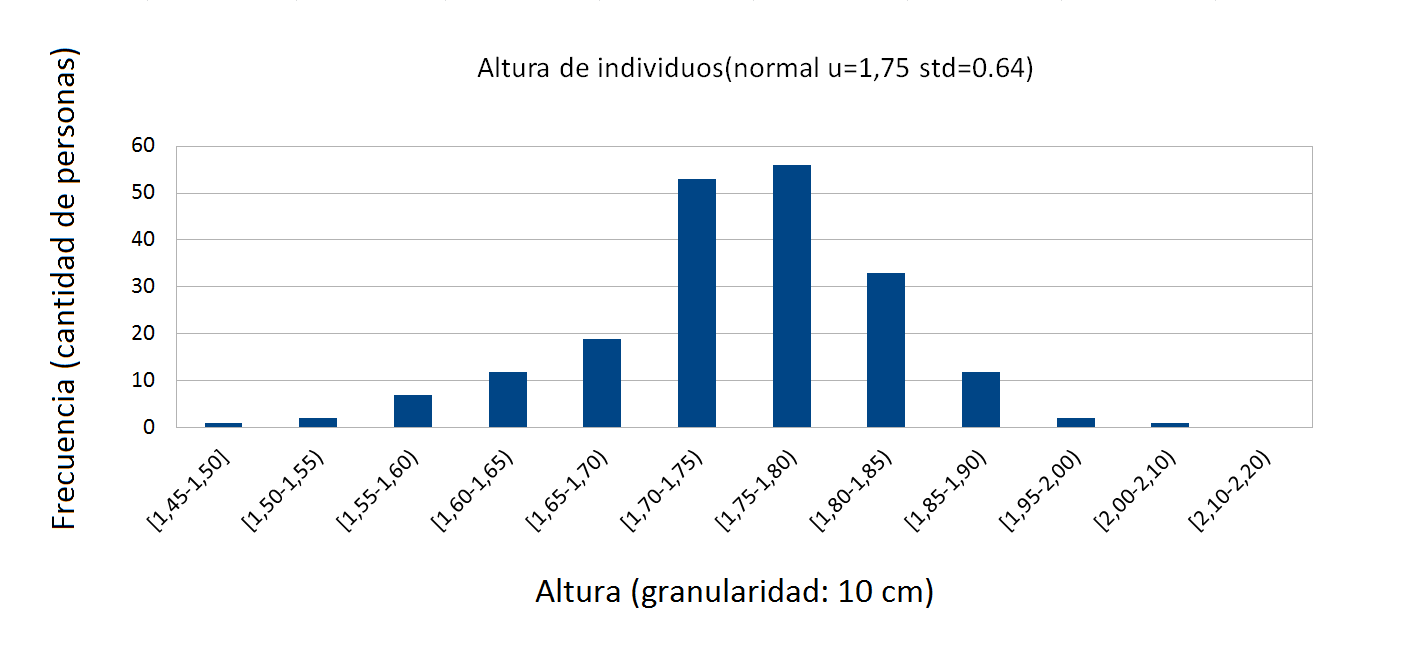
\includegraphics[scale=.41,angle=-90]{imgenes/normal_ejemplo1.png}
	    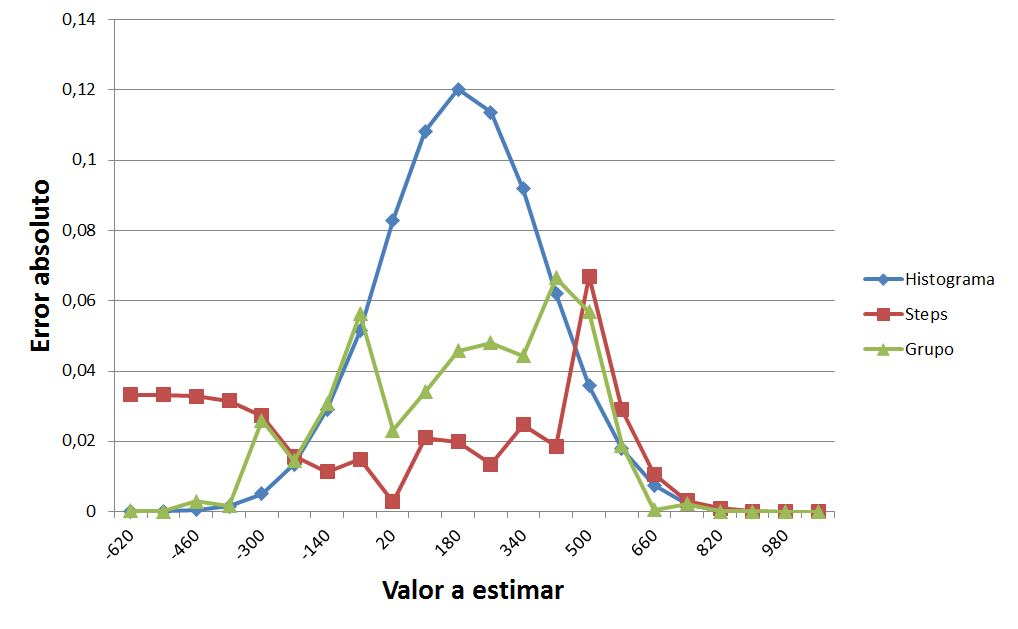
\includegraphics[scale=.55]{imagenes/C2_variando_valor_greater.png}
	    \caption{Errores variando valor a estimar por mayor con par\'ametro fijo} 
	    \label{fig:C2_variando_valor_greater}
	  \end{center}
	\end{figure}
		
		Usando el mismo set de datos uniforme que se uso anteriormente, vemos en la figura \ref{fig:C0_variando_valor_greater} el error de la selectividad pero estimando por mayor. En este caso sucede algo muy parecido a lo que sucede al estimar por igual, con la salvedad de que el de pasos distribuidos no resulta tan constante durante todo el rango.
		
		El error del histograma clasico de nuevo es cada ves mayor a medida que se acerca a la media de la normal. 
		
		El estimador del grupo en esta ocasi\'on resulto ser casi tan bueno como el de pasos distribuidos. Al parecer tiene una buena performance en los datos con distribuci\'on normal.

	\subsubsection{Distribuci\'on uniforme}	

	\quad

\subsubsection*{Caso 3}

	\quad
		
		\begin{tabular}{| l | l |}
		\hline
		Parametro & 20 \\
		\hline
		Columna & C0 \\
		\hline
		Valor minimo & 0 \\
		\hline
		Valor maximo & 999 \\
		\hline
		Distribuci\'on & Uniforme, Media = 4950 \\
		\hline
		Selectividad de & Igualdad \\
		\hline
		\end{tabular}		
		
		\quad
		
		\quad	
						
	\begin{figure}[H]
	  \begin{center}
	    %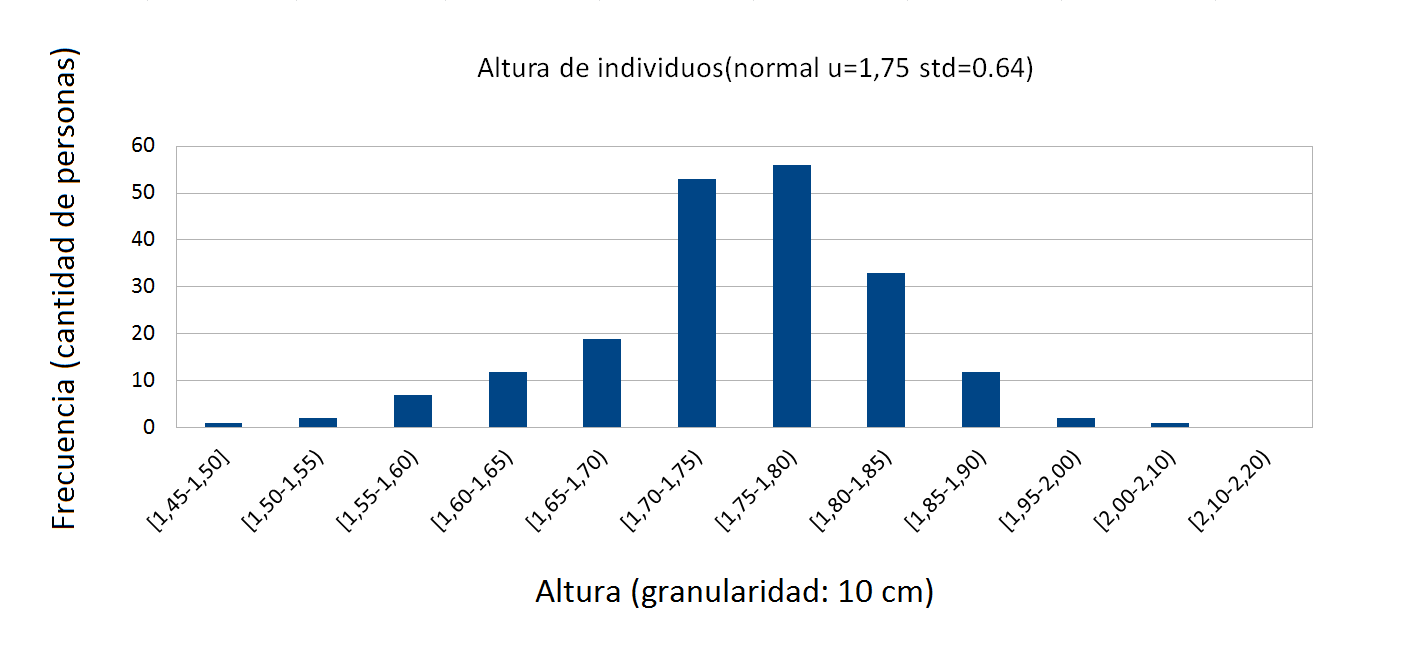
\includegraphics[scale=.41,angle=-90]{imgenes/normal_ejemplo1.png}
	    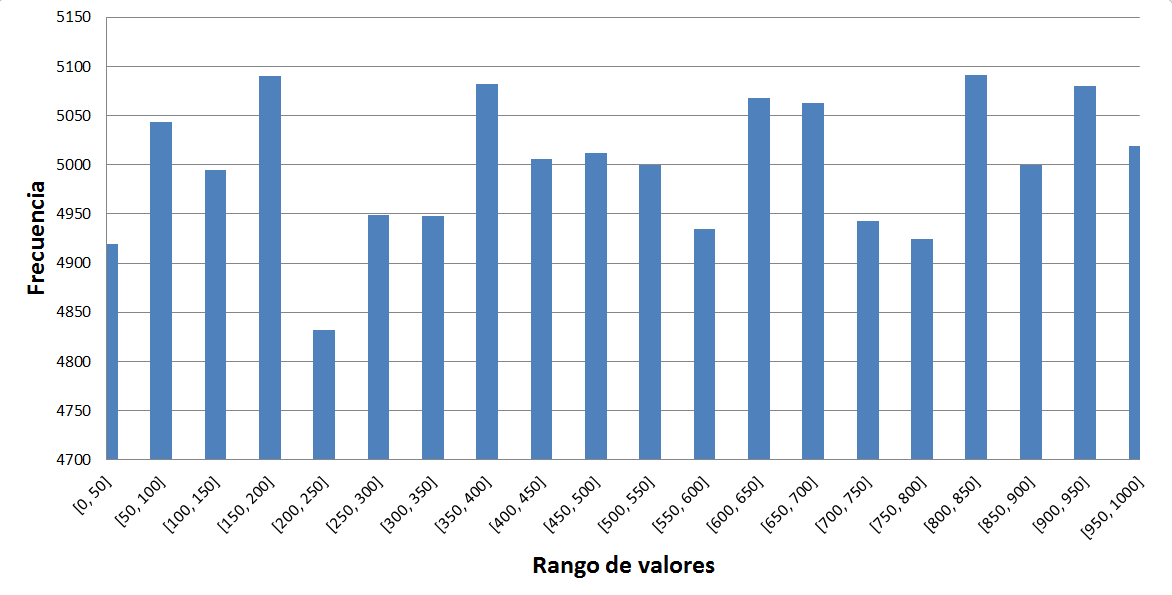
\includegraphics[scale=.50]{imagenes/distro_C0.png}
	    \caption{Gr\'afico de distribuci\'on de la columna C0 del set de datos de la c\'atedra} 
	    \label{fig:(distro_C0}
	  \end{center}
	\end{figure}

	\begin{figure}[H]
	  \begin{center}
	    %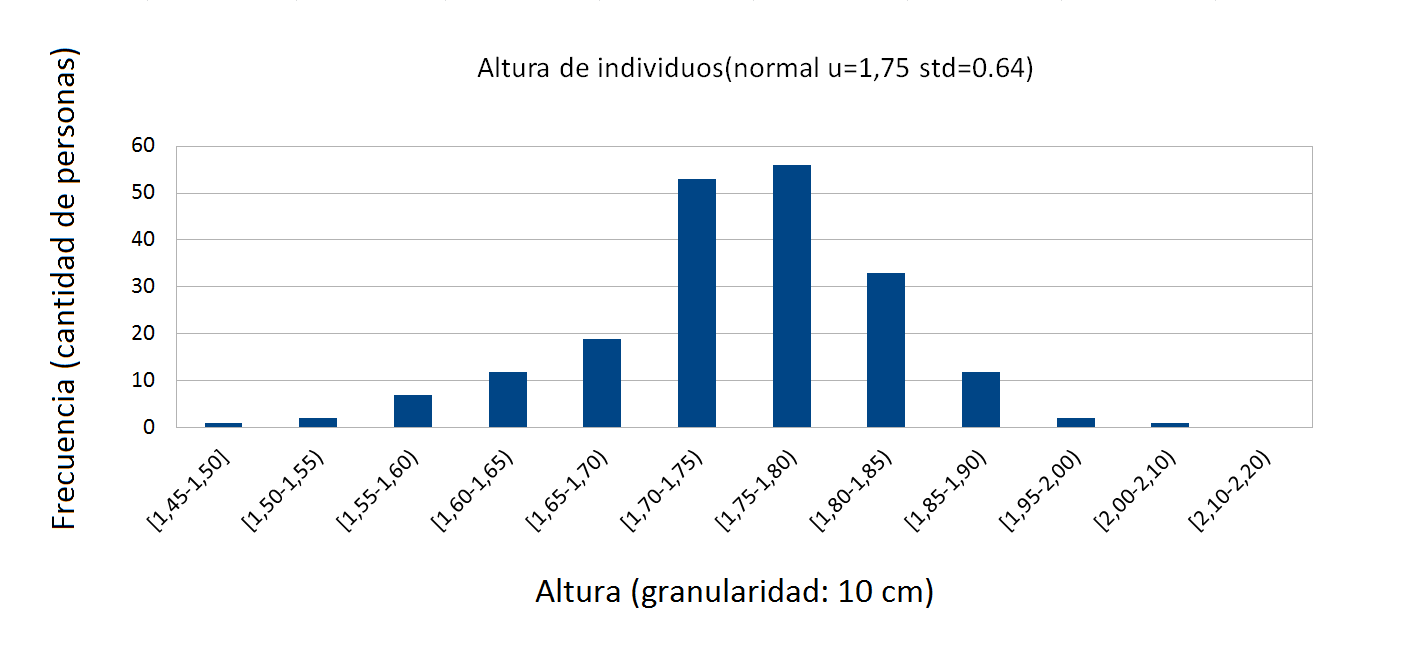
\includegraphics[scale=.41,angle=-90]{imgenes/normal_ejemplo1.png}
	    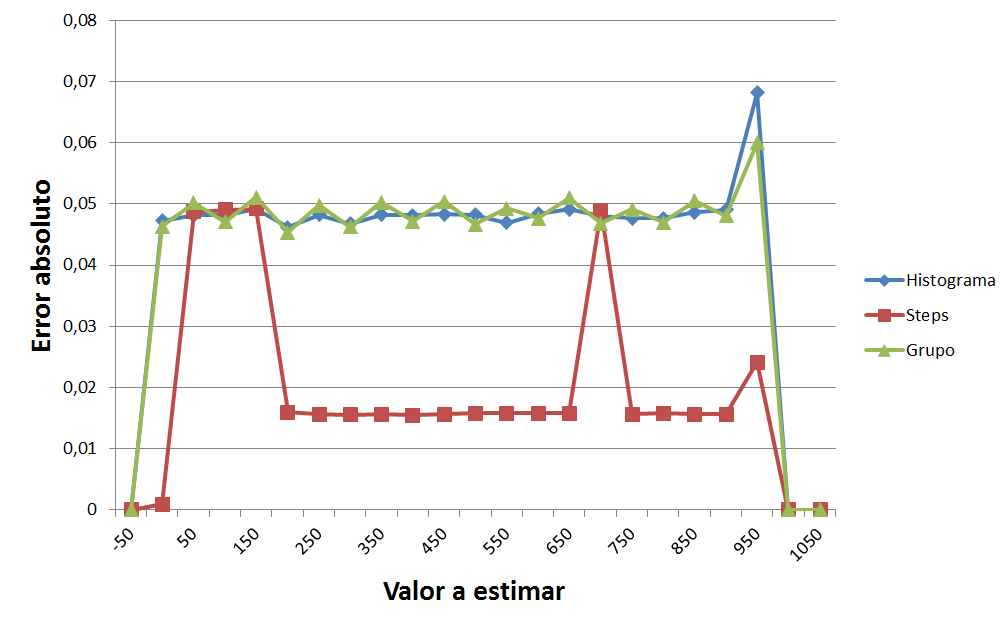
\includegraphics[scale=.60]{imagenes/C0_variando_valor.png}
	    \caption{Errores variando valor a estimar con par\'ametro fijo} 
	    \label{fig:C0_variando_valor}
	  \end{center}
	\end{figure}	
	

		En la figura \ref{fig:(distro_C0} se ve como la distribuci\'on de los datos esta ves es una Uniforme que var\'ia al rededor de 4950.
		
		Seg\'un se ve en la figura \ref{fig:C0_variando_valor}, no hay una gran diferencia esta vez con el Histograma Cl\'asico y el estimador implementado por el grupo. 
		
		En este caso, se puede apreciar como claramente ``Pasos Distribuidos'' obtiene errores bastante menores en casi todo el rango.
		
		Seg\'un pareciese, en los valores donde la distribuci\'on uniforme toma valores altos, los errores de pasos distribuidos aumentan bastante, igualando a los obtenidos en los otros 2 estimadores.

	\newpage

		\subsubsection*{Caso 4}
		
		\begin{tabular}{| l | l |}
		\hline
		Parametro & 20 \\
		\hline
		Columna & C0 \\
		\hline
		Valor minimo & 0 \\
		\hline
		Valor maximo & 999 \\
		\hline
		Distribuci\'on & Uniforme, Media = 4950 \\
		\hline
		Selectividad de & Mayor \\
		\hline
		\end{tabular}	
		
		\quad	

	\begin{figure}[H]
	  \begin{center}
	    %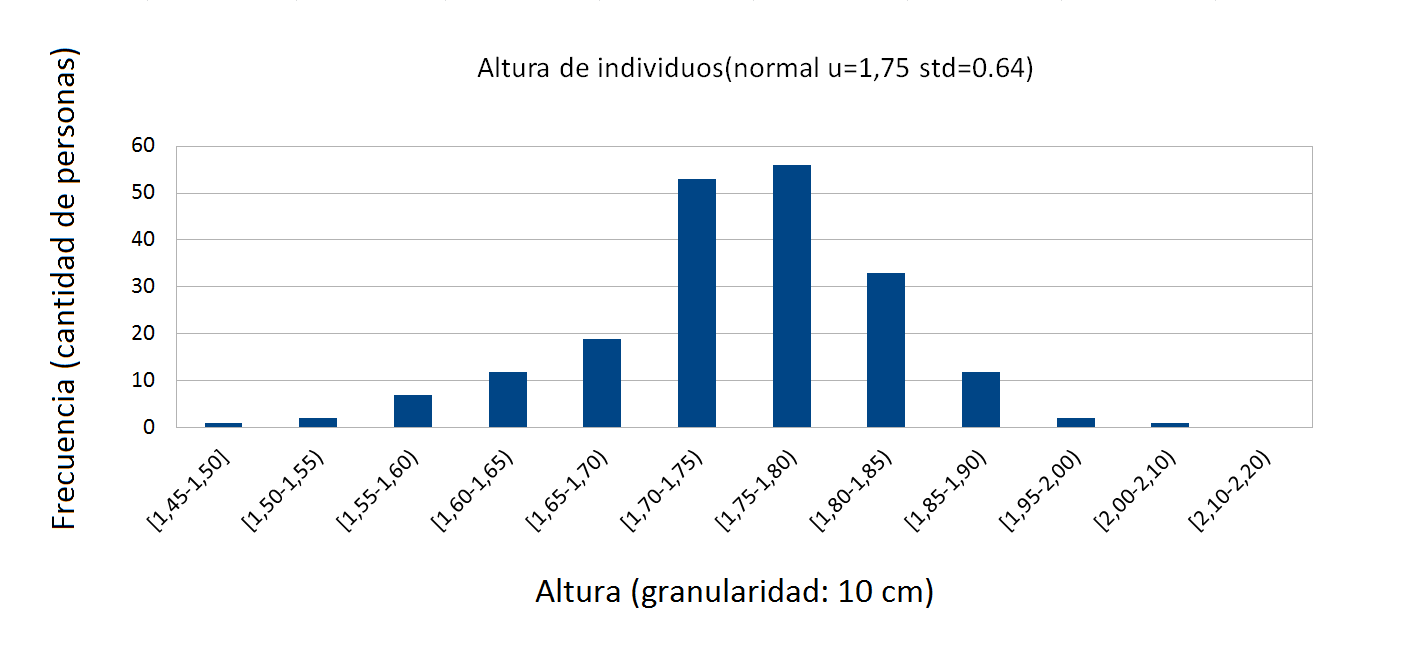
\includegraphics[scale=.41,angle=-90]{imgenes/normal_ejemplo1.png}
	    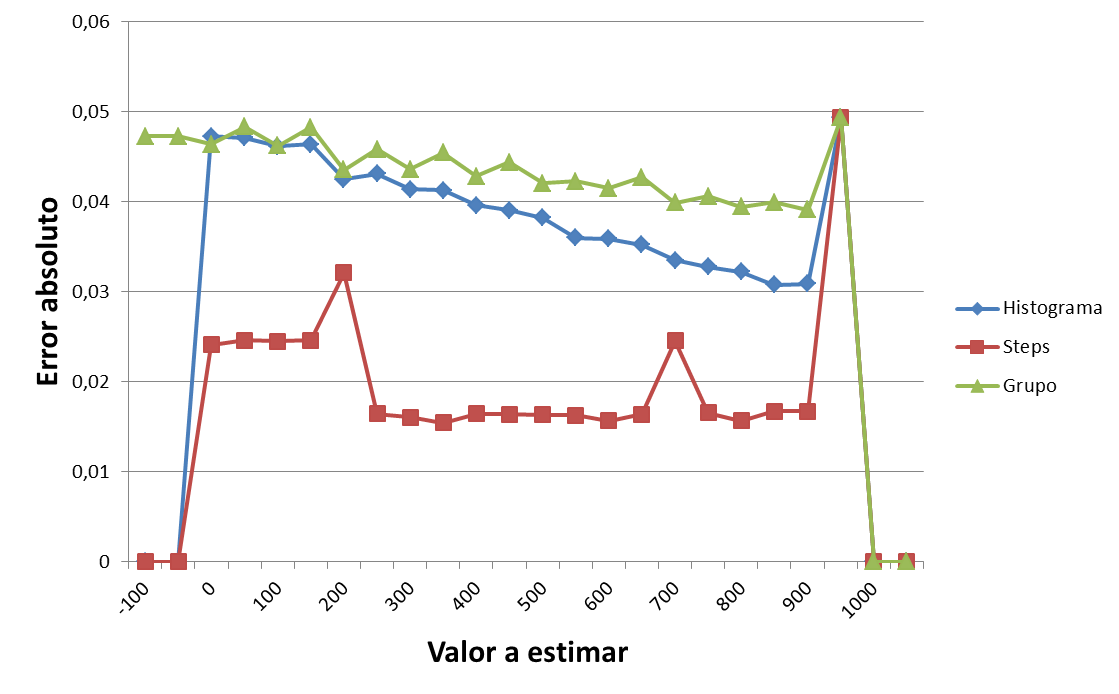
\includegraphics[scale=.55]{imagenes/C0_variando_valor_greater.png}
	    \caption{Errores variando valor a estimar por mayor con par\'ametro fijo} 
	    \label{fig:C0_variando_valor_greater}
	  \end{center}
	\end{figure}	

		En la figura \ref{fig:C0_variando_valor_greater} se realiz\'o un test igual al caso 2, pero estimando por Mayor en vez de por igual. Ya se puede ver como la distribuci\'on es un factor muy importante al momento de utilizar los estimadores.
		
		En este caso, el estimador del grupo fue incluso peor que el histograma cl\'asico, y se ve como la diferencia de error aumenta a medida que se acerca al valor m\'as alto del rango.